\documentclass[12pt, spanish]{article}
\usepackage[spanish]{babel}
\selectlanguage{spanish}
%\usepackage{natbib}
\usepackage{url}
\usepackage[utf8x]{inputenc}
\usepackage{graphicx}
\graphicspath{{images/}}
\usepackage{parskip}
\usepackage{fancyhdr}
\usepackage{vmargin}
\usepackage{multirow}
\usepackage{float}
\usepackage{chngpage}
\usepackage{enumitem}

\usepackage{amsfonts}

\usepackage{subcaption}

\usepackage{hyperref}
\usepackage[
    type={CC},
    modifier={by-nc-sa},
    version={4.0},
]{doclicense}

\hypersetup{
    colorlinks=true,
    linkcolor=blue,
    filecolor=magenta,
    urlcolor=cyan,
}

% para codigo
\usepackage{listings}
\usepackage{xcolor}



%% configuración de listings

\definecolor{listing-background}{HTML}{F7F7F7}
\definecolor{listing-rule}{HTML}{B3B2B3}
\definecolor{listing-numbers}{HTML}{B3B2B3}
\definecolor{listing-text-color}{HTML}{000000}
\definecolor{listing-keyword}{HTML}{435489}
\definecolor{listing-identifier}{HTML}{435489}
\definecolor{listing-string}{HTML}{00999A}
\definecolor{listing-comment}{HTML}{8E8E8E}
\definecolor{listing-javadoc-comment}{HTML}{006CA9}

\lstdefinestyle{eisvogel_listing_style}{
  language         = python,
%$if(listings-disable-line-numbers)$
%  xleftmargin      = 0.6em,
%  framexleftmargin = 0.4em,
%$else$
  numbers          = left,
  xleftmargin      = 0em,
 framexleftmargin = 0em,
%$endif$
  backgroundcolor  = \color{listing-background},
  basicstyle       = \color{listing-text-color}\small\ttfamily{}\linespread{1.15}, % print whole listing small
  breaklines       = true,
  frame            = single,
  framesep         = 0.19em,
  rulecolor        = \color{listing-rule},
  frameround       = ffff,
  tabsize          = 4,
  numberstyle      = \color{listing-numbers},
  aboveskip        = 1.0em,
  belowskip        = 0.1em,
  abovecaptionskip = 0em,
  belowcaptionskip = 1.0em,
  keywordstyle     = \color{listing-keyword}\bfseries,
  classoffset      = 0,
  sensitive        = true,
  identifierstyle  = \color{listing-identifier},
  commentstyle     = \color{listing-comment},
  morecomment      = [s][\color{listing-javadoc-comment}]{/**}{*/},
  stringstyle      = \color{listing-string},
  showstringspaces = false,
  escapeinside     = {/*@}{@*/}, % Allow LaTeX inside these special comments
  literate         =
  {á}{{\'a}}1 {é}{{\'e}}1 {í}{{\'i}}1 {ó}{{\'o}}1 {ú}{{\'u}}1
  {Á}{{\'A}}1 {É}{{\'E}}1 {Í}{{\'I}}1 {Ó}{{\'O}}1 {Ú}{{\'U}}1
  {à}{{\`a}}1 {è}{{\'e}}1 {ì}{{\`i}}1 {ò}{{\`o}}1 {ù}{{\`u}}1
  {À}{{\`A}}1 {È}{{\'E}}1 {Ì}{{\`I}}1 {Ò}{{\`O}}1 {Ù}{{\`U}}1
  {ä}{{\"a}}1 {ë}{{\"e}}1 {ï}{{\"i}}1 {ö}{{\"o}}1 {ü}{{\"u}}1
  {Ä}{{\"A}}1 {Ë}{{\"E}}1 {Ï}{{\"I}}1 {Ö}{{\"O}}1 {Ü}{{\"U}}1
  {â}{{\^a}}1 {ê}{{\^e}}1 {î}{{\^i}}1 {ô}{{\^o}}1 {û}{{\^u}}1
  {Â}{{\^A}}1 {Ê}{{\^E}}1 {Î}{{\^I}}1 {Ô}{{\^O}}1 {Û}{{\^U}}1
  {œ}{{\oe}}1 {Œ}{{\OE}}1 {æ}{{\ae}}1 {Æ}{{\AE}}1 {ß}{{\ss}}1
  {ç}{{\c c}}1 {Ç}{{\c C}}1 {ø}{{\o}}1 {å}{{\r a}}1 {Å}{{\r A}}1
  {€}{{\EUR}}1 {£}{{\pounds}}1 {«}{{\guillemotleft}}1
  {»}{{\guillemotright}}1 {ñ}{{\~n}}1 {Ñ}{{\~N}}1 {¿}{{?`}}1
  {…}{{\ldots}}1 {≥}{{>=}}1 {≤}{{<=}}1 {„}{{\glqq}}1 {“}{{\grqq}}1
  {”}{{''}}1
}
\lstset{style=eisvogel_listing_style}


\usepackage[default]{sourcesanspro}

\setmarginsrb{2 cm}{1 cm}{2 cm}{2 cm}{1 cm}{1.5 cm}{1 cm}{1.5 cm}

\title{Práctica 3:\\
Modelos de Simulación Dinámicos y Discretos.\hspace{0.05cm} }
\author{Antonio David Villegas Yeguas}
\date{\today}

\renewcommand*\contentsname{hola}

\makeatletter
\let\thetitle\@title
\let\theauthor\@author
\let\thedate\@date
\makeatother

\pagestyle{fancy}
\fancyhf{}
\rhead{\theauthor}
\lhead{\thetitle}
\cfoot{\thepage}

\begin{document}

%%%%%%%%%%%%%%%%%%%%%%%%%%%%%%%%%%%%%%%%%%%%%%%%%%%%%%%%%%%%%%%%%%%%%%%%%%%%%%%%%%%%%%%%%

\begin{titlepage}
    \centering
    \vspace*{0.3 cm}
    
\includegraphics[scale = 0.50]{ugr.png}\\[0.7 cm]
    %\textsc{\LARGE Universidad de Granada}\\[2.0 cm]
    \textsc{\large 4º CSI 2020/21 - Grupo 1}\\[0.5 cm]
    \textsc{\large Grado en Ingeniería Informática}\\[0.5 cm]
    \rule{\linewidth}{0.2 mm} \\[0.2 cm]
    { \huge \bfseries \thetitle}\\
    \rule{\linewidth}{0.2 mm} \\[1 cm]

    \begin{minipage}{0.4\textwidth}
        \begin{flushleft} \large
            \emph{Autor:}\\
            \theauthor\\
			 \emph{DNI:}\\
            77021623-M
            \end{flushleft}
            \end{minipage}~
            \begin{minipage}{0.4\textwidth}
            \begin{flushright} \large
            \emph{Asignatura: \\
            Simulación de Sistemas}   \\
            \emph{Correo:}\\
            advy99@correo.ugr.es
        \end{flushright}
    \end{minipage}\\[0.5cm]

    {\large \thedate}\\[0.5cm]
    %{\url{https://github.com/advy99/AA/}}
    {\doclicenseThis}

    \vfill

\end{titlepage}

%%%%%%%%%%%%%%%%%%%%%%%%%%%%%%%%%%%%%%%%%%%%%%%%%%%%%%%%%%%%%%%%%%%%%%%%%%%%%%%%%%%%%%%%%

\tableofcontents
\pagebreak

%%%%%%%%%%%%%%%%%%%%%%%%%%%%%%%%%%%%%%%%%%%%%%%%%%%%%%%%%%%%%%%%%%%%%%%%%%%%%%%%%%%%%%%%%


\section*{Introducción}

Para esta práctica se nos plantean distintos modelos de simulación de cara a conocer las diferencias entre una gestión de tiempo de incremento fijo o variable, así como estudiar el funcionamiento de modelos dinámicos y discretos.

\section{Gestión del tiempo: Métodos de incremento fijo e incremento variable de tiempo}

Este sistema necesita que cierto número de máquinas estén siempre en funcionamiento, de forma que para evitar fallos se dispone de una serie de repuestos. Si una máquina se estropea, se cambia por un repuesto, y se envia a un taller para que la máquina sea reparada, de forma que cuando esté reparada, pasará a formar parte de las máquinas de repuesto.

De esta forma, este sistema se basa en gestionar los estados en los que falla una máquina, se repara, y vuelve de la reparación, de forma que tendremos como parámetros el número de máquinas, el número de reparadores del taller, el tiempo de reparación y el tiempo de fallo, estos dos últimos siguiento una distribución de probabilidad exponencial.


\subsection{Prueba de los dos modelos implementados}

Tras desarrollar ambos modelos he realizado las pruebas pedidas en el guión de prácticas, de cara a comparar las ejecuciones, obteniendo los siguientes resultados:

\begin{table}[H]
\begin{tabular}{|c|c|c|c|c|c|}
\hline
\multicolumn{6}{|c|}{\textbf{Sistema de tiempo fijo}}                                          \\ \hline
T. reparacion & T. fallo & D. fallos & N. fallos & D. media fallos & D. media fallos teorica \\ \hline
0.5           & 1        & 0         & 4091      & 0               & 0                       \\ \hline
2             & 1        & 4441      & 2905      & 1.52874         & 2                       \\ \hline
12            & 24       & 1251      & 113       & 11.0708         & 12.0325                 \\ \hline
48            & 24       & 5559      & 107       & 51.9533         & 48.3043                 \\ \hline
720           & 1440     & 584       & 1         & 584             & 833.25                  \\ \hline
2880          & 1440     & 1118      & 1         & 1118            & 3333							\\ \hline
\end{tabular}
\end{table}

\begin{table}[H]
\begin{tabular}{|c|c|c|c|c|c|}
\hline
\multicolumn{6}{|c|}{\textbf{Sistema de tiempo variable}}                                      \\ \hline
T. reparacion & T. fallo & D. fallos & N. fallos & D. media fallos & D. media fallos teorica \\ \hline
0.5           & 1        & 0         & 0         & 0               & 0                       \\ \hline
2             & 1        & 5684.44   & 2864      & 1.98479         & 2                       \\ \hline
12            & 24       & 1297.14   & 105       & 12.3537         & 12                      \\ \hline
48            & 24       & 5570.06   & 110       & 50.637          & 48                      \\ \hline
720           & 1440     & 584.044   & 1         & 584.044         & 720                     \\ \hline
2880          & 1440     & 1118.76   & 2         & 559.381         & 2880							\\ \hline
\end{tabular}
\end{table}


Vemos como en general el sistema que utiliza la variación de tiempo variable se ajusta mejor a los resultados que teoricamente deberíamos obtener, ya que a diferencia del sistema de incremento fijo, se mueve al punto exacto donde ocurre el suceso, mientras que si en el sistema de tiempo fijo ocurre un suceso en el intervalo en el que no se modifica el reloj, no se gestiona hasta el siguiente avance del reloj.

También vemos que si utilizamos medidas más precisas de tiempo, este problema se va solucionando, y es que el espacio de muestreo del reloj fijo es mayor, evitando el problema, ya que, por ejemplo, si usamos un día, pasará de un día a otro, cuando un evento puede ocurrir al inicio del día, mientras que al usar horas o minutos, puede gestionar el suceso en ese espacio muestral más amplio.


\subsection{Comparación de eficiencia entre ambos modelos}

Por último, comprobaremos que sistema es más rápido a la hora de la ejecución. Probando con un gran número de días se ha obtenido lo siguiente:

\begin{figure}[H]
  \centering
      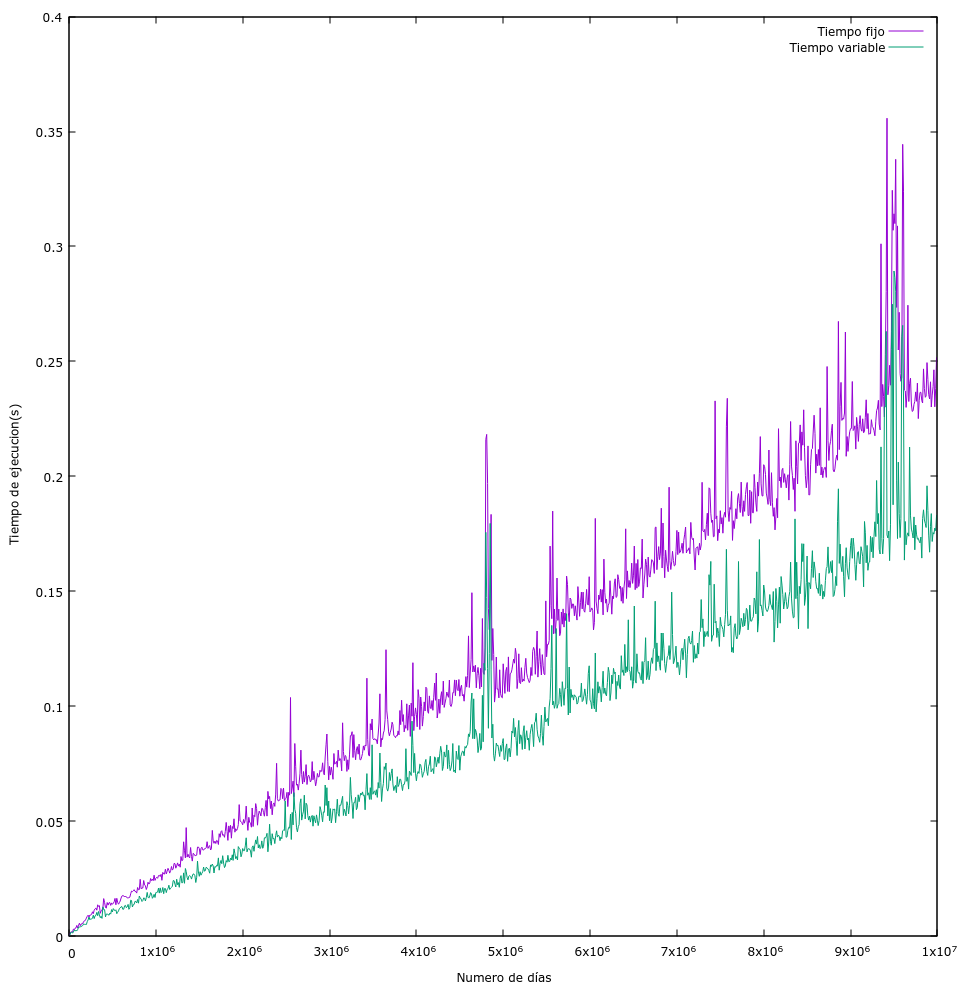
\includegraphics[width=\textwidth]{t1_eficiencia.png}
 		\caption{Comparación de tiempo de ejecución entre el sistema que usa tiempo fijo contra el de tiempo variable.}
\end{figure}


Vemos que el sistema de tiempo fijo, como era de esperar, se comporta peor que el sistema de tiempo variable, y es que el sistema de tiempo fijo en el tiempo que no tiene ningún evento tiene que seguir actualizando su reloj, mientras que el sistema de tiempo variable salta al siguiente evento directamente, evitandose esos ciclos que unicamente incrementa el reloj.


\section{Sucesos y grafos de sucesos: Estructura de un programa de simulación dinámico y discreto}

En este apartado trabajaremos con un sistema similar al anterior, pero en este caso nos centraremos en como funciona su grafo de sucesos, así como en sus parámetros óptimos.

Para este modelo, el número de máquinas y repuestos será variable y nos centraremos en probar distintas configuraciones de cara a comparar si es mejor un sistema con varios reparadores o un único reparador.


Para realizar esta tarea he fijado el número de máquinas a diez y el número de repuestos a dos, es decir, en total doce máquinas, mientras que el tiempo de reparación será de un día y seis horas, y el tiempo de fallo será de un día.


% Please add the following required packages to your document preamble:
% \usepackage{graphicx}
\begin{table}[H]
\centering
\resizebox{\textwidth}{!}{%
\begin{tabular}{|c|c|c|c|c|c|}
\hline
\multicolumn{6}{|c|}{\textbf{Comparación del sistema variando el número de reparadores}}                                                                                                                                                                                          \\ \hline
\textbf{N. reparadores} & \textbf{D. media fallos} & \textbf{T. medio entre fallos} & \textbf{\begin{tabular}[c]{@{}c@{}}N. medio maquinas \\ en reparación\end{tabular}} & \textbf{P. tiempo ocio} & \textbf{\begin{tabular}[c]{@{}c@{}}P. duración total\\ fallos\end{tabular}} \\ \hline
1                       & 364.638                  & 0                              & 11.140                                                                              & 0.038                   & 99.901                                                                      \\ \hline
2                       & 364.868                  & 0                              & 10.250                                                                              & 0.011                   & 99.964                                                                      \\ \hline
3                       & 364.868                  & 0                              & 9.526                                                                               & 0.019                   & 99.964                                                                      \\ \hline
4                       & 90.872                   & 0.460                          & 8.622                                                                               & 0.339                   & 99.595                                                                      \\ \hline
5                       & 24.181                   & 0.154                          & 7.760                                                                               & 1.708                   & 99.374                                                                      \\ \hline
6                       & 14.459                   & 0.141                          & 7.302                                                                               & 5.431                   & 99.034                                                                      \\ \hline
7                       & 16.449                   & 0.142                          & 6.677                                                                               & 12.531                  & 99.147                                                                      \\ \hline
8                       & 7.624                    & 0.142                          & 6.548                                                                               & 21.254                  & 98.177                                                                      \\ \hline
9                       & 10.908                   & 0.151                          & 6.412                                                                               & 29.160                  & 98.620                                                                      \\ \hline
10                      & 12.944                   & 0.091                          & 6.536                                                                               & 34.707                  & 99.293                                                                      \\ \hline
\end{tabular}%
}
\end{table}


Vemos como en este caso, aunque se mantega un gran porcentaje de ocupación por parte de los reparadores al tener los fallos con menor tiempo que lo que suelen tardar en reparar una máquina, el tener más reparadores permite que el tiempo que se tiene de media con fallos baje desde la totalidad de la simulación, a solo unos cuantos días, por lo que los sistemas no resultan equivalentes, y con esto estamos demostrando la gran ayuda que aportan los reparadores, y que estos estén en un gran número si se tarda más en reparar una máquina que en lo que suele tardar en fallar.

Aun así vemos que ya en los últimos casos donde hay muchos reparadores, aunque estén ocupados depende de la aleatoriedad de como se rompan las máquinas, lo que hace que en el tiempo medio de fallos pueda parecer que al final sube, pero en realidad es por la aleatoriedad del sistema. Como vemos, esto no pasa en el porcentaje de tiempo libre, que siempre se incrementa, al haber más reparadores.

Por último para este apartado, como nos pide el guión, la configuración con la que conseguimos mantener el porcentaje de duración total de fallos por debajo de un 10\% es la siguiente:

\begin{lstlisting}
Con 1 repuestos y 3 reparadores se ha conseguido que el porcentaje total de fallos esté por debajo de un 89.382 por ciento del tiempo
\end{lstlisting}

Además, en el script adjunto a la práctica aparecerán más configuraciones que consiguen rebajar aún más este porcentaje.

\subsection{Modificación del modelo original}

También se nos pide realizar una modificación al sistema, de forma que se añada un suceso de mantenimiento (con su respectivo fin de mantenimiento), de cara a que si hay algún reparador libre, revise las máquinas para que tarden más en estropearse.

De cara a desarrollar y comprobar este apartado simplemente se han añadido dichos estados al código, con sus respectivas funciones que realizan lo indicado en el grafo de sucesos del guión, y se ha ejecutado con los mismos parámetros que el apartado anterior, añadiendo un tiempo de revisión de un día, y un tiempo de reparación uniforme entre dos horas y media y veinte horas.

Con esto obtenemos los siguientes resultados:

\begin{lstlisting}
Con 1 repuestos y 2 reparadores se ha conseguido que el porcentaje total de fallos esté por debajo de un 88.890 por ciento
\end{lstlisting}

Que como vemos, ha mejorado el anterior, necesitando un reparador menos. Además tambien podemos ver que con la misma cantidad de reparadores, se obtiene un resultado mucho mejor:

\begin{lstlisting}
Con 1 repuestos y 3 reparadores se ha conseguido que el porcentaje total de fallos esté por debajo de un 38.880 por ciento
\end{lstlisting}



\section{Mi tercer modelo de simulación discreto}

\section{Análisis de salidas y experimentación}

% \begin{thebibliography}{9}
%
%
% \end{thebibliography}

\end{document}
